\documentclass[a4paper,11pt]{article}
\pdfoutput=1 % if your are submitting a pdflatex (i.e. if you have
             % images in pdf, png or jpg format)

\usepackage{jinstpub} % for details on the use of the package, please
                      % see the JINST-author-manual

\usepackage{lineno}
\linenumbers

\newcommand{\vtrxp}{VTRx+}

\title{Development of a high bandwidth readout chain for the CMS Phase-2 pixel upgrade}

%% %simple case: multiple authors, same institution
\author{C. Smith}
\affiliation{The University of Kansas,\\Lawrence, Kansas 66045, USA}

% \affiliation{The University of Kansas\\1251 Wescoe Hall Dr.\\Lawrence, KS 66045, United States}

% From CMS publication:
% The University of Kansas, Lawrence, Kansas 66045, USA
% From KU physics website:
% The University of Kansas, 1251 Wescoe Hall Dr. Lawrence, KS 66045, United States

% more complex case: 4 authors, 3 institutions, 2 footnotes
% \author[a,b,1]{F. Irst,\note{Corresponding author.}}
% \author[c]{S. Econd,}
% \author[a,2]{T. Hird\note{Also at Some University.}}
% \author[c,2]{and Fourth}

% The "\note" macro will give a warning: "Ignoring empty anchor..."
% you can safely ignore it.

% \affiliation[a]{One University,\\some-street, Country}
% \affiliation[b]{Another University,\\different-address, Country}
% \affiliation[c]{A School for Advanced Studies,\\some-location, Country}

% e-mail addresses: only for the corresponding author
\emailAdd{caleb.smith@ku.edu}

\abstract{
The CMS collaboration is building a new inner tracking pixel detector for the High-Luminosity LHC.
Each pixel readout chip will be controlled with a single serial input stream at 160 Mbps and will send out data via four CML 1.28 Gbps outputs.
The readout chips will be grouped in modules and connected with up to 1.6 m long low-mass electrical links to Low-Power Gigabit Transceivers (lpGBT) and Versatile Link PLUS Transceivers (\vtrxp) modules that send the data optically to off-detector electronics at 10 Gbps.
The development and the characterization of these components is presented along with system tests of the readout chain.
}

\keywords{Only keywords from JINST's keywords list please}

% \arxivnumber{1234.56789} % only if you have one

% \collaboration{\includegraphics[height=17mm]{example-image}\\[6pt]
%   XXX collaboration}
% or
\collaboration[c]{on behalf of the CMS collaboration}


% if you write for a special issue this may be useful
\proceeding{Topical Workshop on Electronics for Particle Physics\\
  September 20--24, 2021\\
  Online event}

\begin{document}
\maketitle
\flushbottom

% Comment on abbreviations
% We suggest not to abbreviate: ``section'', ``appendix'', ``figure''
% and ``table'', but ``eq.'' and ``ref.'' are welcome. Also, please do
% not use \texttt{\textbackslash emph} or \texttt{\textbackslash it} for
% latin abbreviaitons: i.e., et al., e.g., vs., etc.

\section{Introduction}
\label{sec:introduction}

The High-Luminosity LHC (HL-LHC) will provide CMS with a peak instantaneous luminosity of $7.5 \times 10^{34} \mathrm{cm}^{-2} \mathrm{s}^{-1}$ starting in 2027.
Compared to the LHC, the HL-LHC will have up to 200 proton-proton collisions (pileup) per event and will shower CMS with a higher radiation fluence.
To prepare for this data taking environment, the CMS Tracker will be fully replaced in the Phase-2 upgrade~\cite{ref:tdr,ref:orfanelli}.

The new inner tracker will have about two billion silicon pixels installed.
The detector will be built using hybrid pixel modules, and the sensor data will be processed by a custom readout chip (ROC) developed by the RD53 collaboration~\cite{ref:rd53}.
Each frontend readout chip needs a control link to receive trigger, clock, commands, and settings from backend electronics as well as a data links to send pixel data to backend electronics.
The high bandwidth control and data links are split into two stages: electrical links and optical links.
System tests of electrical and optical links are presented.

\section{Data Readout Chain}
\label{sec:readout}

An overview of the data readout chain for the inner tracker is shown in figure~\ref{fig:readout}.
High bandwidth electrical and optical links are used to establish control and data links between pixel modules on the CMS detector and Data Trigger Control (DTC) boards in the counting room.
Low-mass electronic links (e-links) up to 1.6 meters long provide 160 Mpbs control links (downlinks) and 1.28 Gbps data links (uplinks) between pixel modules and portcards.
Optical fibers connect portcards, which are mounted on the support structure inside the detector, to DTCs in the counting room to establish 2.5 Gbps control links (downlinks) and 10 Gbps data links (uplinks).
The portcards are printed circuit boards that each carry three Low-Power Gigabit Transceivers (lpGBT) and three Versatile Link PLUS Transceivers (\vtrxp) modules~\cite{ref:lpgbt,ref:vtrxp}.
The lpGBTs convert optical signals to electrical signals (and vise versa), and the \vtrxp\space modules establish optical links with the DTCs.

\begin{figure}[htbp]
\centering
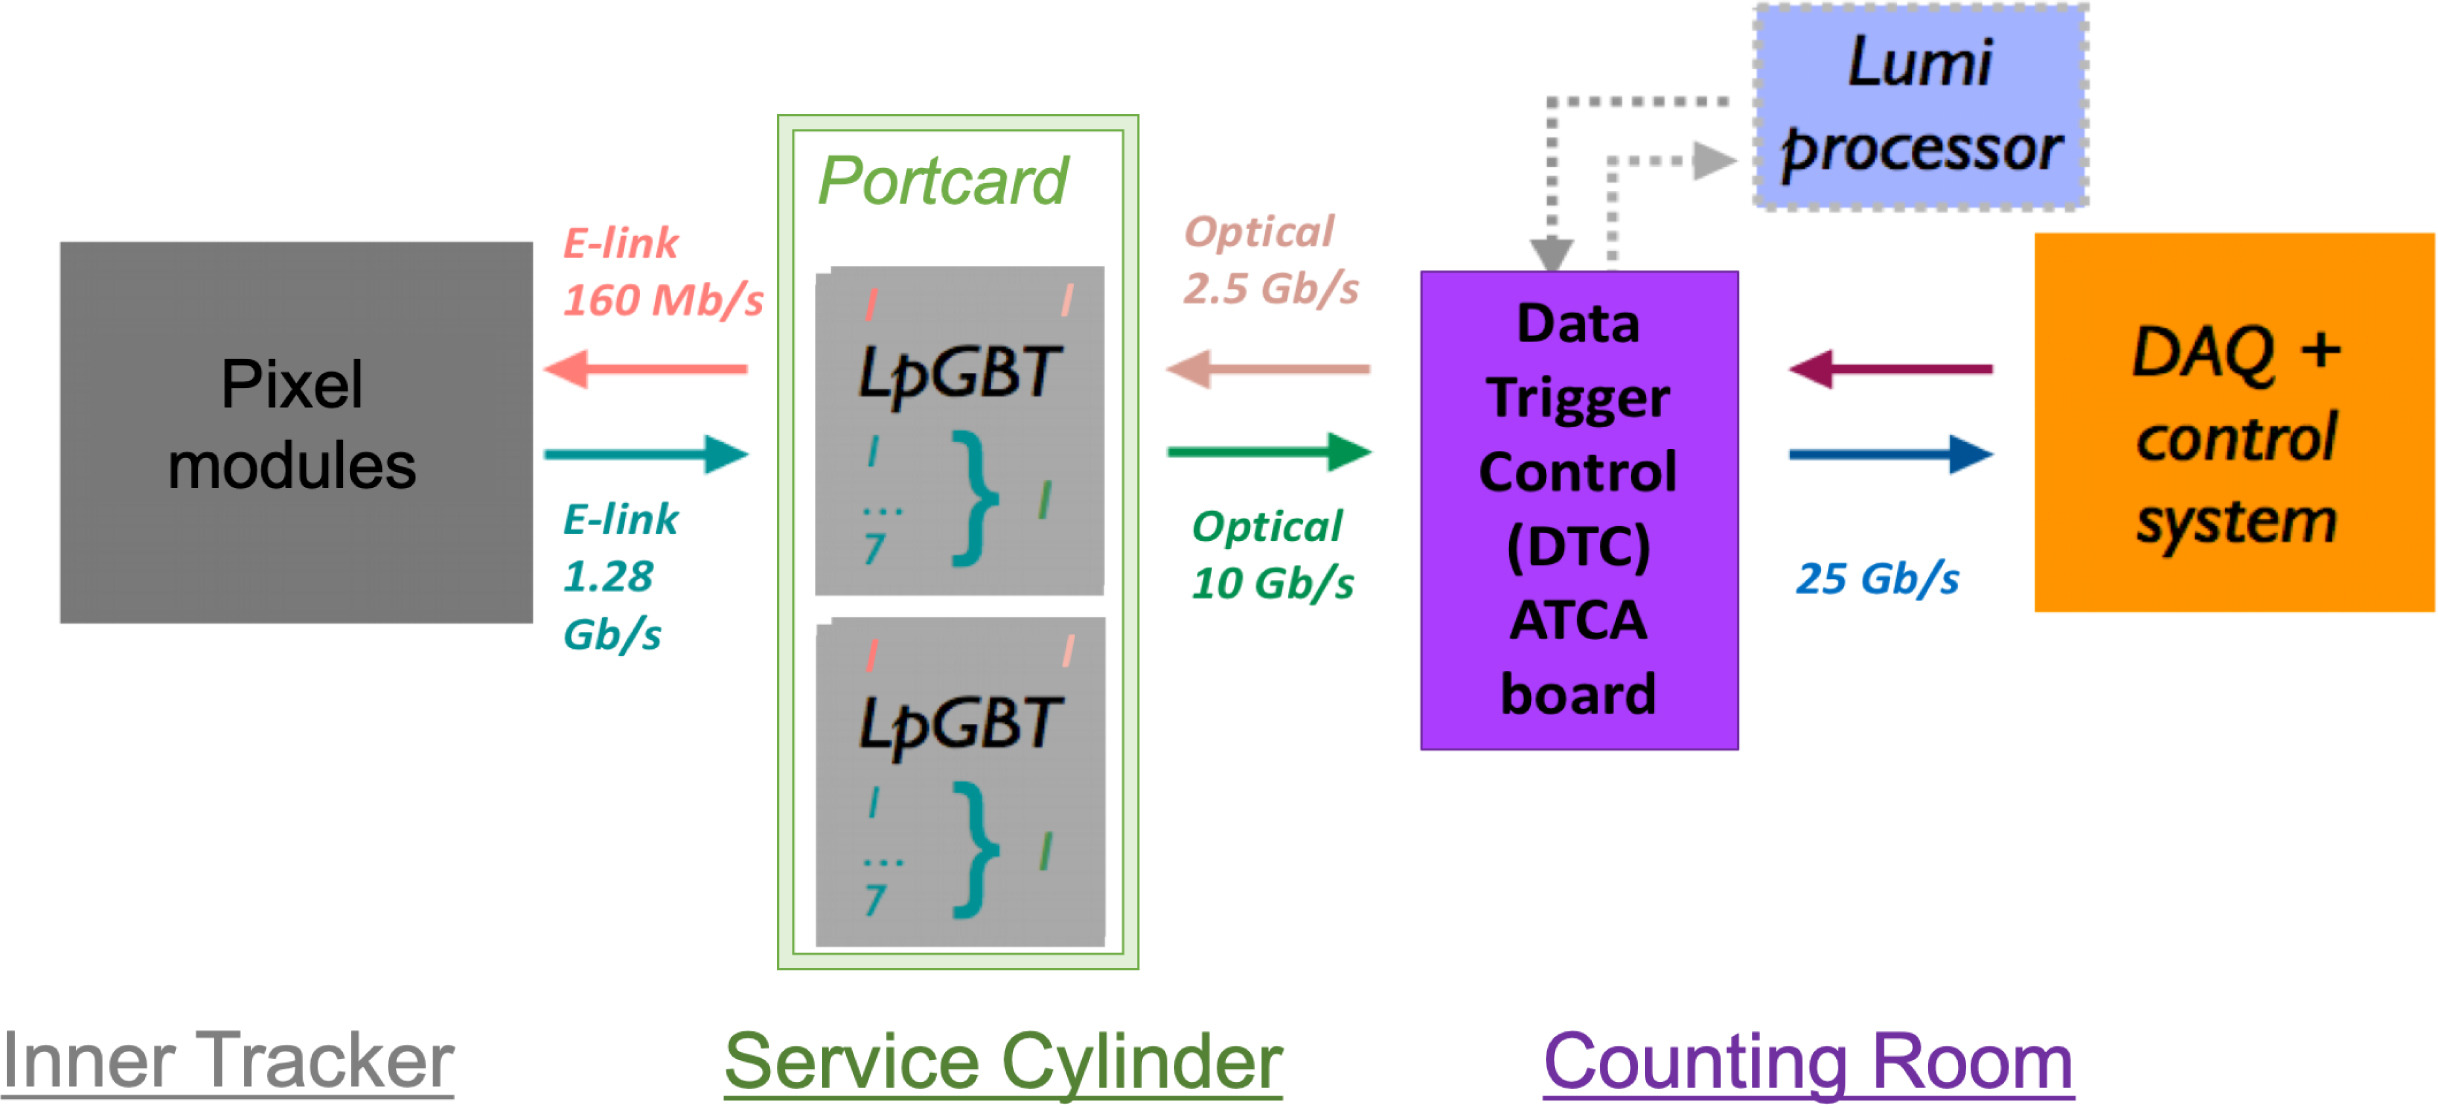
\includegraphics[width=1.0\textwidth,origin=c]{../figures/IT_System_Readout.jpg}
\caption{
\label{fig:readout}
System readout architecture for the inner tracker. Pixel modules communicate with portcards through e-links. Portcards communicate with DTCs through optical links.
}
\end{figure}

\section{Electrical Links}
\label{sec:electrical}

% =============
% E-link design
% =============

% Describe e-link design and reasons for design choices.

% Info
%
% Each wire has a 36 AWG copper core (127 microns in diameter) surrounded by a polyimide coating for insolation (45 micron thickness); the total diameter is 217 microns.
%
% Polyimide braiding is used to lash twisted pairs in a bundle to provide durability and prevent wire kinks.
%
% Different epoxies tested: Araldite 2011 and UR 6060.
% Final epoxy used: UR 6060.
%
% Different gauges tested: 34 and 36 AWG.
% Final gauge used: 36 AWG.
%
% Different twists per inch tested: 3, 4, 6, 8, 16, 24.
% Final twists per inch used: 4.

One end of a twisted pair electrical link (e-link) is shown in figure~\ref{fig:elink}.
Five twisted pair channels (one for a control link and four for data links) are lashed together in a bundle using a polyimide braiding.
The lashing provides durability and prevents wire kinks.
Each twisted pair has two wires that are twisted together with 4 twists per inch.
On each end of an e-link, wires are soldered to a paddle board, and a nonconductive epoxy (UR 6060) is applied to secure the wires.
Each wire has a 36 AWG copper core (127 microns in diameter) surrounded by a polyimide coating for insolation (45 micron thickness); the total diameter is 217 microns.

\begin{figure}[htbp]
\centering
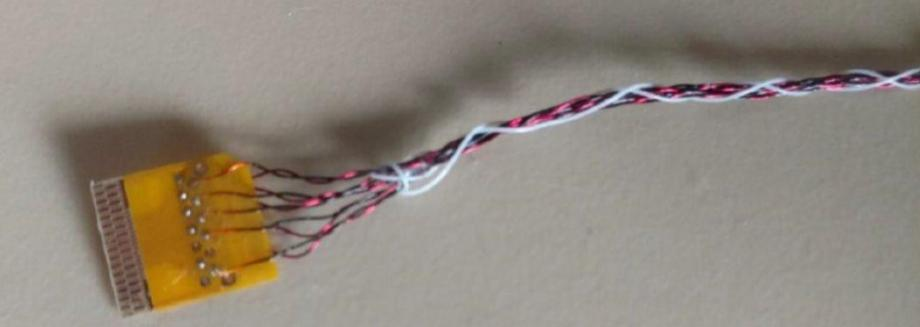
\includegraphics[width=0.5\textwidth,origin=c]{../figures/e-link-1.jpg}
\caption{
\label{fig:elink}
One end of a twisted pair electrical link (e-link).
}
\end{figure}

% ==============
% E-link testing
% ==============

% TODO: expand description of tests

% The tests performed on e-links are continuity, visual inspection, mass measurement, DC resistance, differential eye diagram, bit error rate tests (BERT), impedance measurements, cross talk, thermal cycling, and radiation.

The prototype low-mass electrical links are being developed and characterized with a series of measurements.
The signal quality is assessed using eye diagrams to quantify the amplitude and jitter as well as identifying any distortion.
Bit error rate scans are using to characterize signal integrity across e-links.
Cross talk effects from channels within an e-link bundle and from multiple bundles is studied.
The RD53 chip on a Single Chip Card (SCC) is readout over e-links using an FC7.
Bit error rates are measured using the RD53 chip, and different signal amplitudes for the RD53 are tested to quantify the effect on the error rate.

Radiation testing was performed to determine if e-links can maintain performance in a high radiation environment.
Two different epoxies, Araldite 2011 and UR 6060, were used for e-links that underwent radiation testing.
For doses up to 1300 Mrad, the Araldite 2011 epoxy showed significant darkening, while the UR 6060 epoxy remained clear and transparent.
The signal integrity on e-links remained good after radiation doses.
The polyimide braiding used for lashing becomes brittle after 1900 MRad, but this should not effect the electrical readout.

% ==================
% E-link performance
% ==================

The readout of the RD53A chip across e-links is tested using an FC7, as shown in figure~\ref{fig:tap0_vs_length}.
E-links of two gauges (34 and 36 AWG) and different lengths (0.35 to 2.0 meters).
Bit error rates are determined using a pseudorandom bitstream (PRBS).
The RD53 signal amplitude is varied using the TAP0 setting.
Longer e-links require a larger signal amplitude to maintain a given bit error rate.
Good performance is seen for e-links up to 2.0 meters.

\begin{figure}[htbp]
\centering
\includegraphics[width=0.5\textwidth,origin=c]{../figures/fc7_elink_scc_setup.jpg}
\qquad
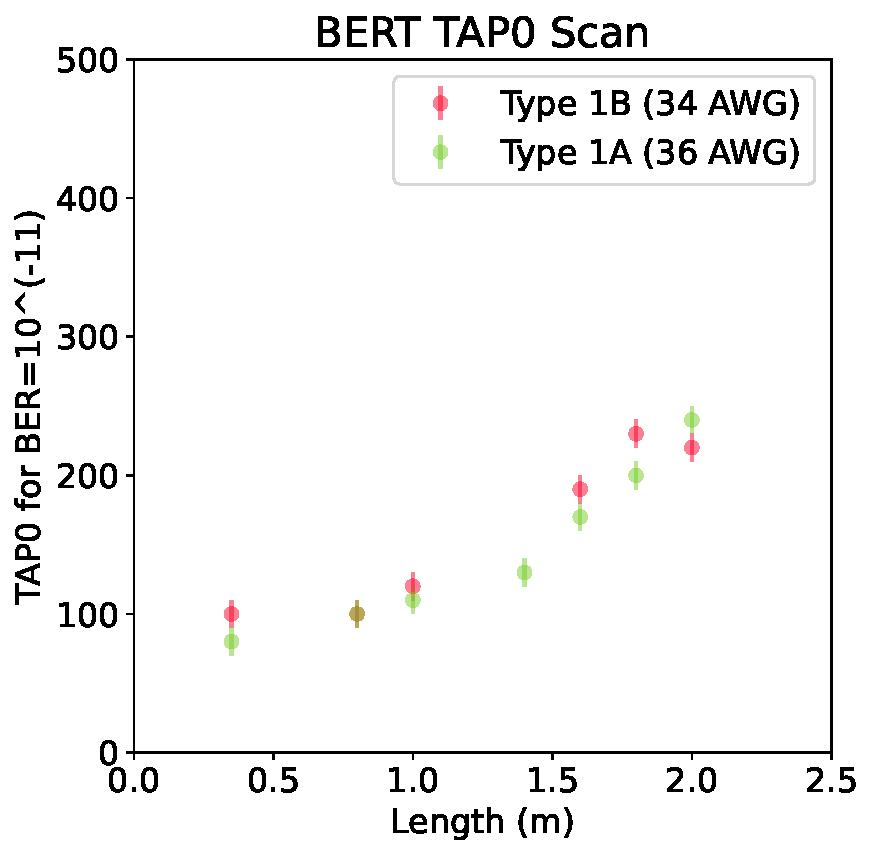
\includegraphics[width=0.4\textwidth,origin=c]{../figures/BERT_TAP0_vs_Length.pdf}
\caption{
\label{fig:tap0_vs_length}
Measurement of signal amplitude (set by TAP0) for electrical links as a function of e-link length for 34 and 36 AWG e-links.
In the hardware setup (left), an FC7 is connected to an SCC through two commercial DP cables, an adapter board, and an e-link for control and readout communication of an RD53A chip.
The measurements (right) show the TAP0 setting to achieve a bit error rate of $10^{-11}$ errors per second for e-links of different lengths.
% For e-links of different lengths, the TAP0 setting to achieve a bit error rate of $10^{-11}$ errors per second is measured (right).
% The necessary signal amplitude increases with e-link length as expected.
% Good performance is seen for e-links up to 2.0 meters.
}
\end{figure}

% Crosstalk measurements

An external crosstalk measurement was performed, and the results are shown in figure~\ref{fig:external_crosstalk}.
To mitigate the effect of external crosstalk from a large aggressor amplitude, the victim amplitude set by TAP0 only requires a small increase.
Thus, external crosstalk from the single aggressor e-link has a small effect on readout over the victim e-link.

\begin{figure}[htbp]
\centering
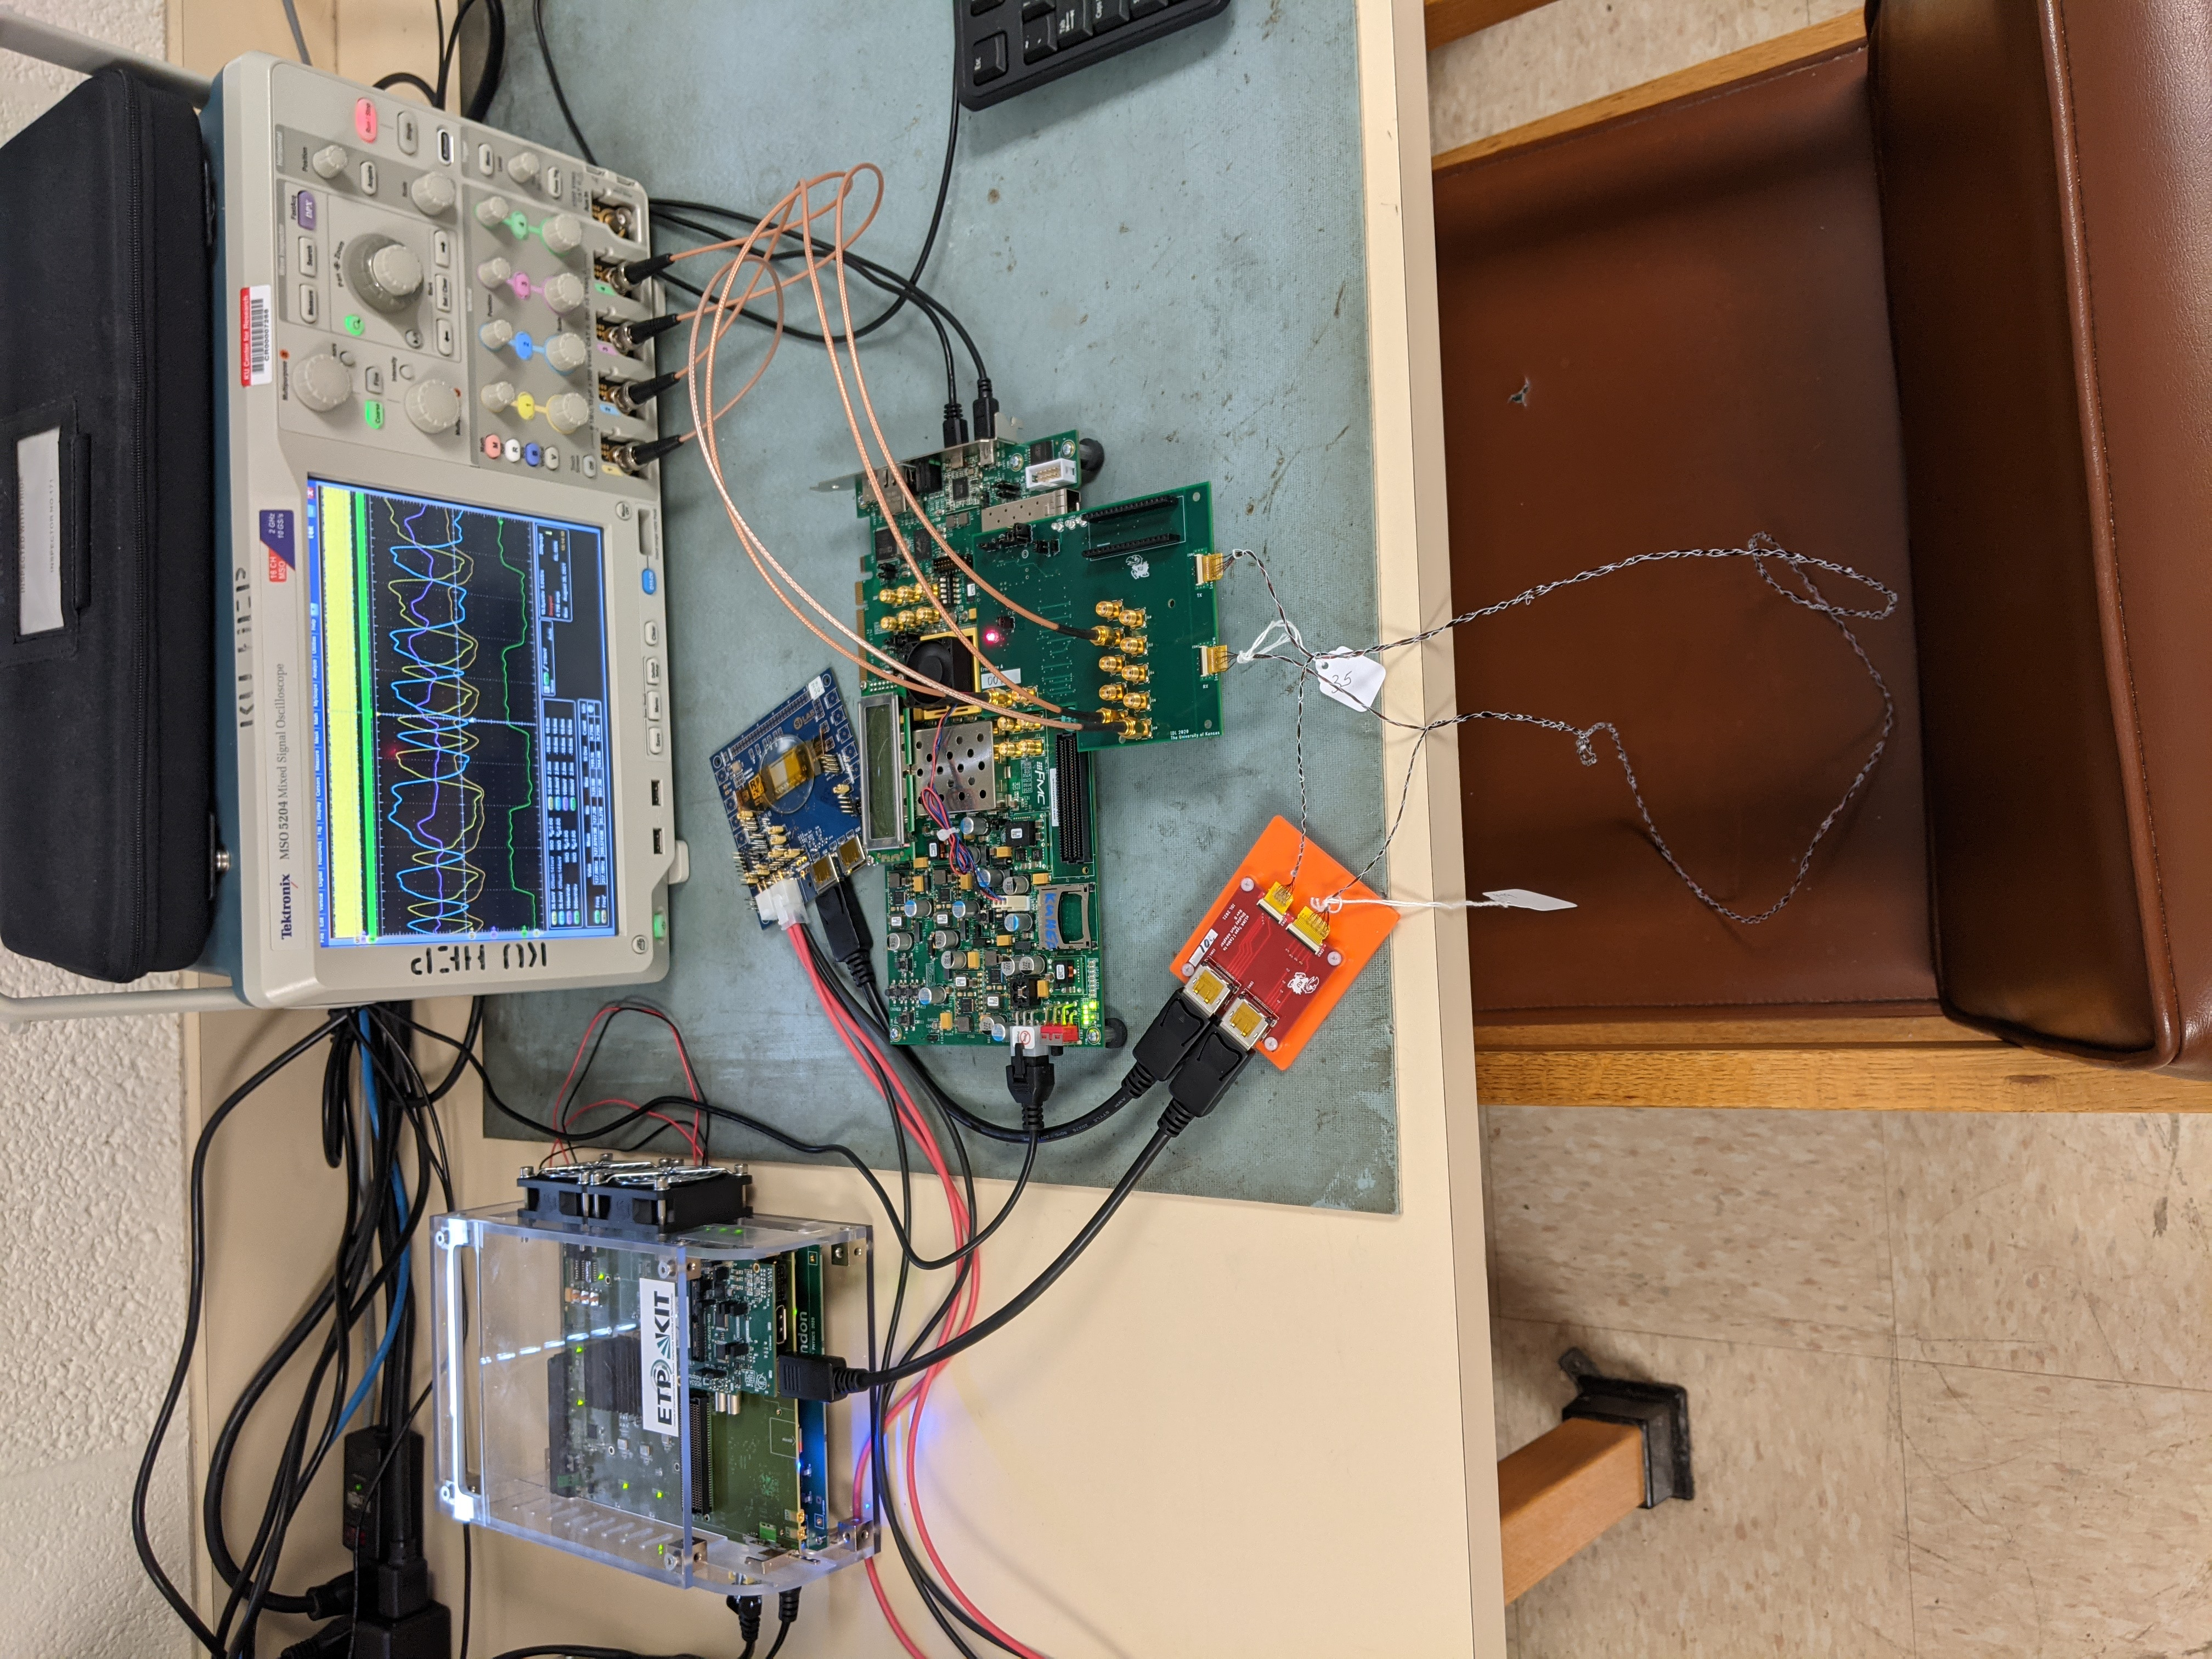
\includegraphics[width=0.5\textwidth,origin=c,angle=270]{../figures/external_crosstalk_setup.jpg}
\qquad
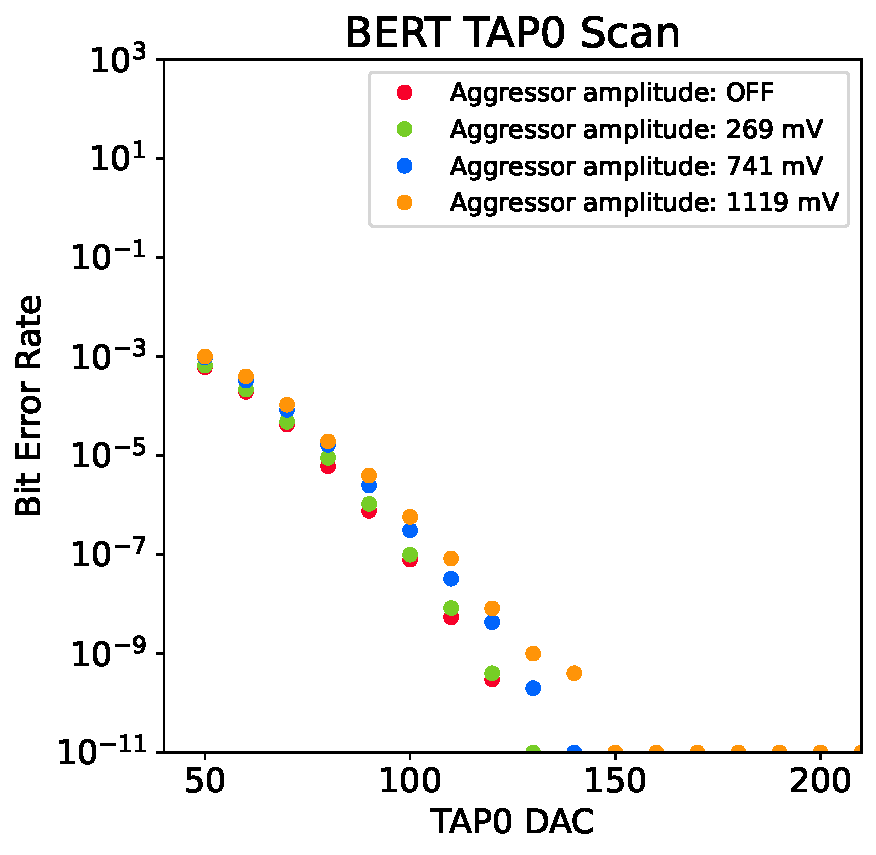
\includegraphics[width=0.5\textwidth,origin=c]{../figures/BERT_TAP0_Scan_External_Crosstalk.pdf}
\caption{
\label{fig:external_crosstalk}
Measurement of the effect of external crosstalk on data transmission.
Two e-links (1.4 meters, 36 AWG) are twisted together (left), with a victim e-link connected between an FC7 and SCC to readout from an RD53A chip, and an aggressor e-link connected to a KC705.
The KC705 sends PRBS signals on four e-link channels on the aggressor at different amplitudes.
}
\end{figure}

\section{Portcards with Optical Links}
\label{sec:optical}

Dedicated setups with the portcards reading out single ROC cards with short coaxial cables have been used to test the prototype portcard and validate the optical part of the readout chain.

See figure~\ref{fig:port_card_design}.

See figure~\ref{fig:port_card_pics}.

\begin{figure}[htbp]
\centering
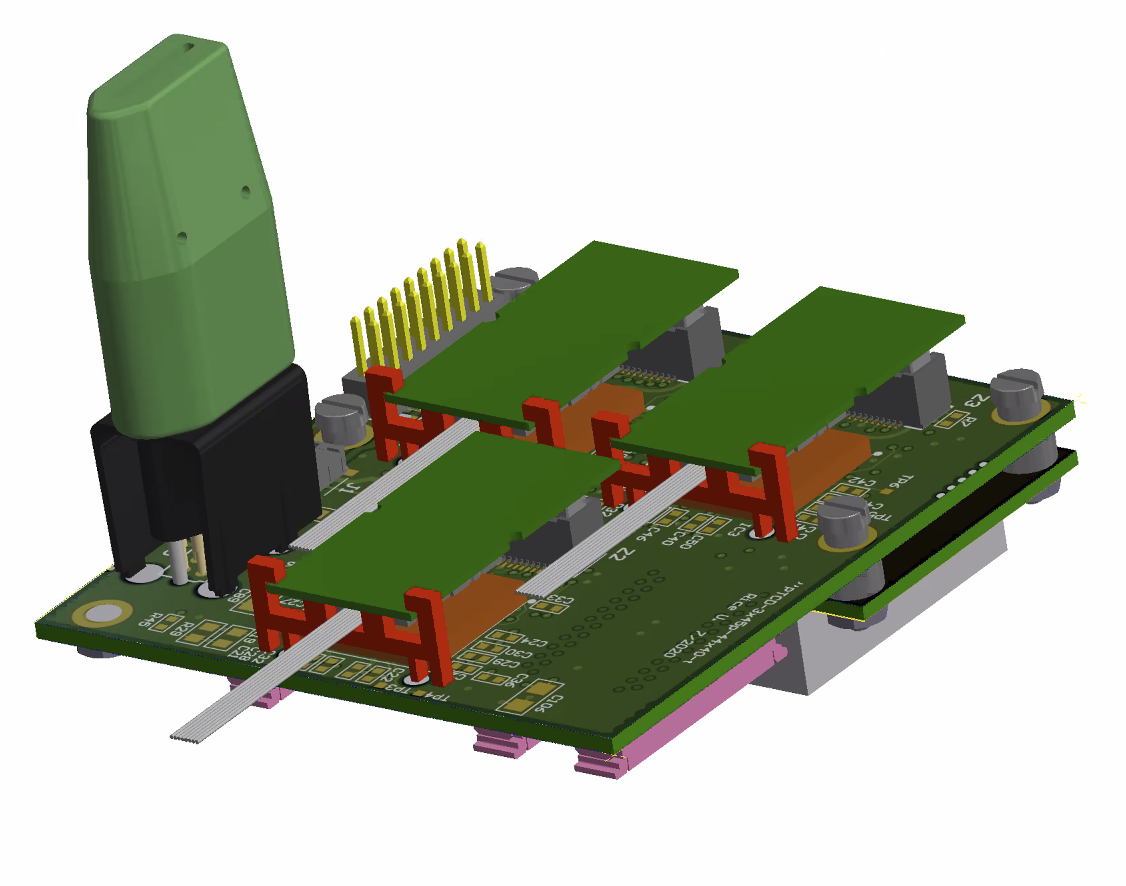
\includegraphics[width=0.5\textwidth,origin=c]{../figures/port_card_design.png}
\caption{
\label{fig:port_card_design}
Portcard design.
}
\end{figure}

\begin{figure}[htbp]
\centering
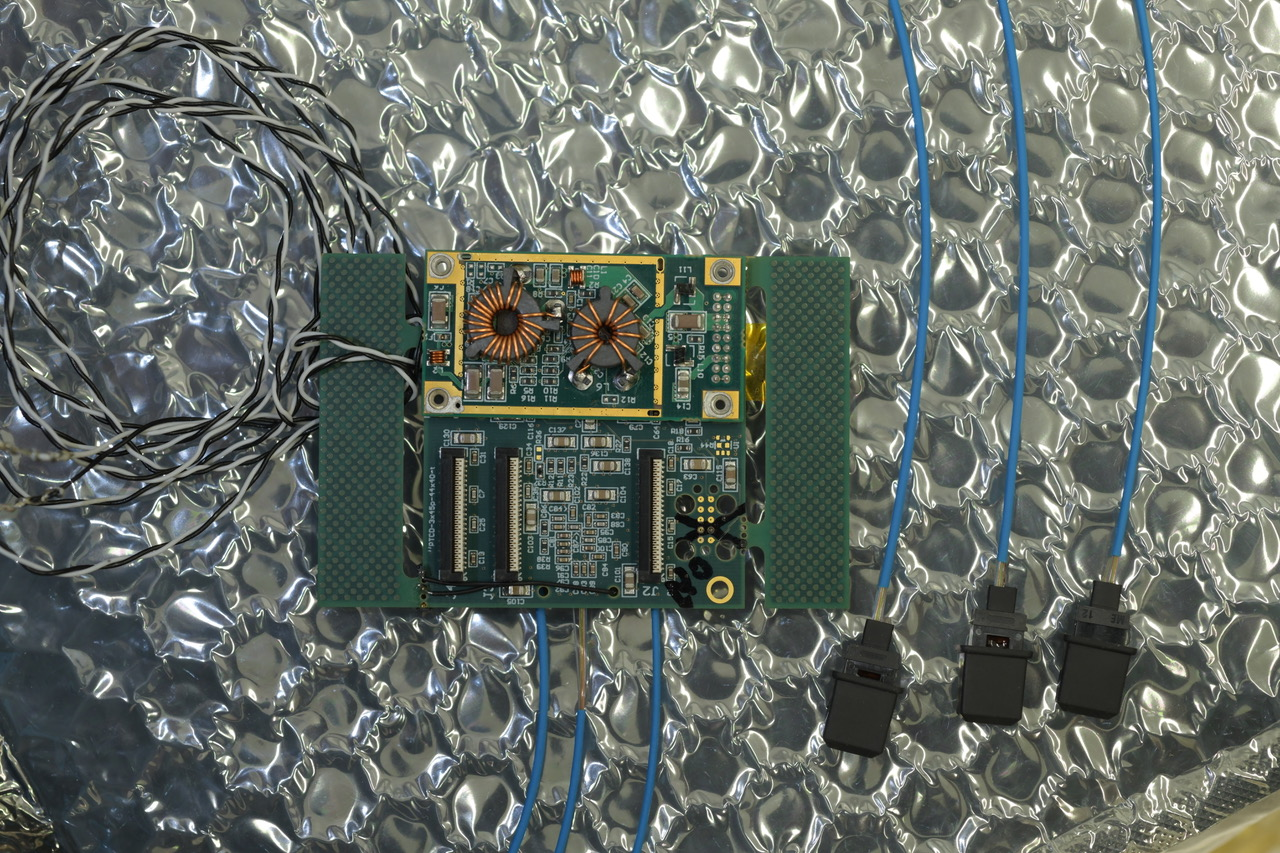
\includegraphics[width=0.45\textwidth,origin=c]{../figures/port_card_front.jpeg}
\qquad
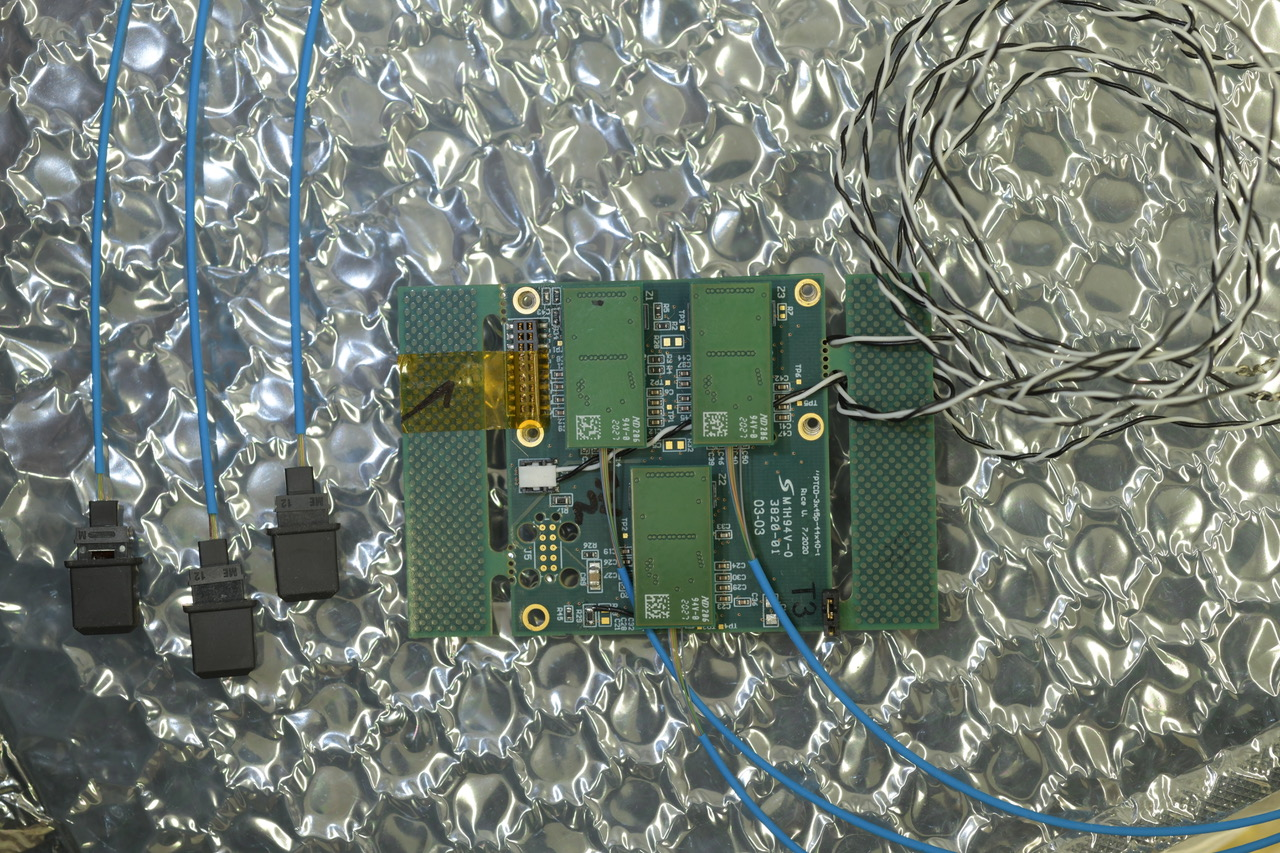
\includegraphics[width=0.45\textwidth,origin=c]{../figures/port_card_back.jpeg}
\caption{
\label{fig:port_card_pics}
Portcard photos.
}
\end{figure}

See figure~\ref{fig:lpgbt_eye}.

See figure~\ref{fig:lpgbt_bert}.

\begin{figure}[htbp]
\centering
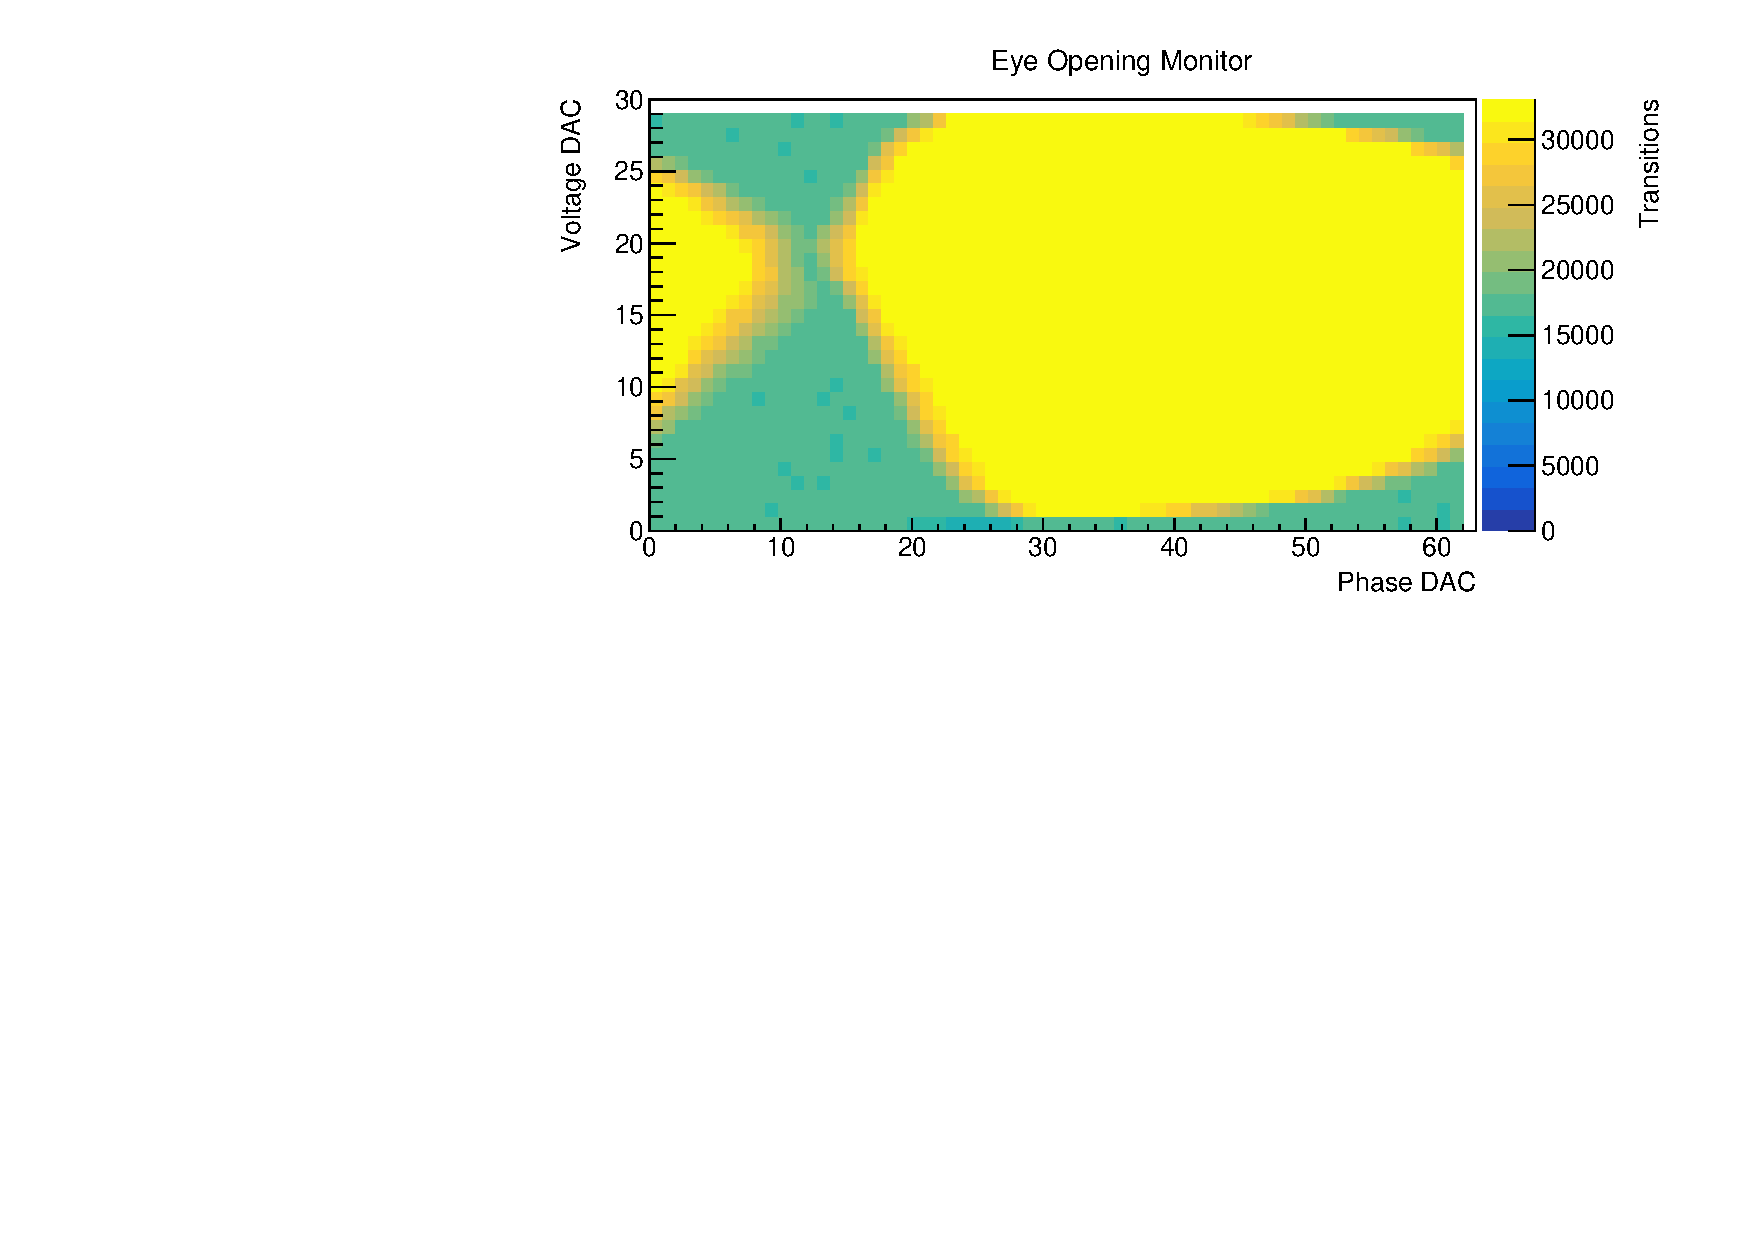
\includegraphics[width=0.5\textwidth,origin=c]{../figures/lpGBT_eye.pdf}
\caption{
\label{fig:lpgbt_eye}
Eye opening monitor from an lpGBT for the 2.56 Gbps optical down link.
The plot shows the height of the eye as a function of sampling phase.
The high-speed input to the lpGBT is compared to a variable (5-bit), fixed voltage by a comparator sampled with a phase interpolated clock.
Transitions of the comparator are counted; within the eye the output should toggle, above or below no transitions are expected.
The color scale shows the number of transitions.
The region with high toggle count corresponds to the eye opening.
Equalization parameters are at default settings.
}
\end{figure}

\begin{figure}[htbp]
\centering
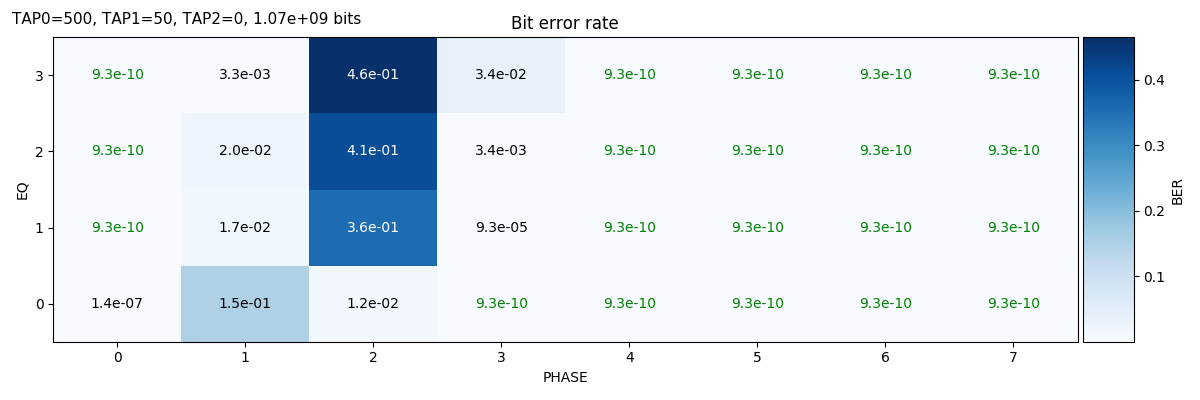
\includegraphics[width=1.0\textwidth,origin=c]{../figures/lpGBT_bert.png}
\caption{
\label{fig:lpgbt_bert}
Scan of bit-error rate vs. clock sampling phase and equalization setting for e-port receivers on the lpGBT driven by the RD53A pixel readout chip over commercial DP cable, adapter and Molex FPC cables.
The source is a PRBS7 generator in the RD53A read out chip, compared to the internal error checker in the lpGBT.
Points in green have zero observed errors and report the reciprocal of the number of bits checked.
The phase at the eye crossing is clearly seen.
Equalization settings affect the timing slightly.
}
\end{figure}

\section{Conclusion}
\label{sec:conclusion}

The data readout chain is an important part of the CMS Phase-2 pixel upgrade.
Various system tests have been performed to characterize the electrical and optical links that form the readout chain.
Electrical links can provide stable links at the required lengths, and crosstalk has a small effect on signal quality.
Conversion from electrical to optical links is working well, and the optical links have good performance.
% Current studies demonstrate good performance of electrical and optical links.
These results will inform the final design, production, and testing of components for the pixel detector readout chain.

% Appendices
% \appendix
% \section{Example appendix title}
% Here is this appendix.

\acknowledgments

The author would like to thank the National Science Foundation for funding this research.

% We suggest to always provide author, title and journal data:
% in short all the informations that clearly identify a document.

\begin{thebibliography}{99}

% TDR Ref.
%
% @techreport{CERN-LHCC-2017-009,
%       title         = "{The Phase-2 Upgrade of the CMS Tracker}",
%       institution   = "CERN",
%       collaboration = "CMS Collaboration",
%       address       = "Geneva",
%       reportNumber  = "CERN-LHCC-2017-009, CMS-TDR-014",
%       month         = "Jun",
%       year          = "2017",
%       url           = "https://cds.cern.ch/record/2272264",
% }

\bibitem{ref:tdr}
CMS Collaboration, \emph{The Phase-2 Upgrade of the CMS Tracker},
CERN-LHCC-2017-009 (2017).

% S. Orfanelli Ref.
%
% @article{ORFANELLI2020164396,
% 	abstract = {A new silicon tracker will be built for the Phase 2 Upgrade of the CMS experiment to fully exploit the increased luminosity delivered by the HL-LHC. The innermost part, called the Inner Tracker, will be exposed to extreme conditions such as unprecedented radiation levels of 1.2Grad and 2.3×1016 neq/cm2 and hit rate of 3.2GHz/cm2. The new Inner Tracker relies on many novel solutions and technologies that allow for a design of a light and radiation-hard pixel detector of high performance. The hybrid pixel modules will be composed of pixel sensors with pixel size of 2500μm2 and a new ASIC, designed in 65 nm CMOS technology, developed by the RD53 collaboration. A novel scheme of serial powering will be deployed to power the pixel modules and new technologies will be used for a high bandwidth readout system. The mechanics will be lightweight, based on carbon-fibre material and two-phase CO2 cooling. In this contribution, the design of the CMS Inner Tracker system will be presented along with the prospective design choices.},
% 	author = {S. Orfanelli},
% 	doi = {https://doi.org/10.1016/j.nima.2020.164396},
% 	issn = {0168-9002},
% 	journal = {Nuclear Instruments and Methods in Physics Research Section A: Accelerators, Spectrometers, Detectors and Associated Equipment},
% 	keywords = {Silicon detectors, Inner tracker, Readout electronics, Serial powering},
% 	pages = {164396},
% 	title = {The Phase 2 Upgrade of the CMS Inner Tracker},
% 	url = {https://www.sciencedirect.com/science/article/pii/S0168900220307932},
% 	volume = {980},
% 	year = {2020},
% 	Bdsk-Url-1 = {https://www.sciencedirect.com/science/article/pii/S0168900220307932},
% 	Bdsk-Url-2 = {https://doi.org/10.1016/j.nima.2020.164396}
% }

\bibitem{ref:orfanelli}
S. Orfanelli, \emph{The Phase 2 Upgrade of the CMS Inner Tracker},
Nuclear Instruments and Methods in Physics Research Section A: Accelerators, Spectrometers, Detectors and Associated Equipment (2020).

% RD53 Ref.
%
% @techreport{Garcia-Sciveres:2287593,
%       author        = "Garcia-Sciveres, Maurice",
%       title         = "{The RD53A Integrated Circuit}",
%       institution   = "CERN",
%       collaboration = "RD53 Collaboration",
%       address       = "Geneva",
%       reportNumber  = "CERN-RD53-PUB-17-001",
%       month         = "Oct",
%       year          = "2017",
%       url           = "https://cds.cern.ch/record/2287593",
% }

\bibitem{ref:rd53}
M. Garcia-Sciveres, \emph{The RD53A Integrated Circuit},
CERN-RD53-PUB-17-001 (2017).

% VTRx+ Ref.
%
% @article{So_s_2017,
% 	abstract = {The Versatile Link PLUS project targets the phase II upgrades of the ATLAS and CMS experiments. It will develop a radiation resistant optical link, operating at up to 10 Gb/s in the upstream and up to 5 Gb/s in the downstream directions with a smaller footprint and higher channel count than its predecessor. A low-profile package is being developed that allows volume production at reduced costs, but which nevertheless can be configured to suit the individual channel count needs of different detectors. This paper describes the development strategies and summarizes the status of the feasibility demonstration phase of the project.},
% 	author = {C. So{\'{o}}s and S. D{\'{e}}traz and L. Olanter{\"a} and C. Sigaud and J. Troska and F. Vasey and M. Zeiler},
% 	doi = {10.1088/1748-0221/12/03/c03068},
% 	journal = {Journal of Instrumentation},
% 	month = {mar},
% 	number = {03},
% 	pages = {C03068--C03068},
% 	publisher = {{IOP} Publishing},
% 	title = {Versatile Link {PLUS} transceiver development},
% 	url = {https://doi.org/10.1088/1748-0221/12/03/c03068},
% 	volume = {12},
% 	year = 2017,
% 	Bdsk-Url-1 = {https://doi.org/10.1088/1748-0221/12/03/c03068}
% }

\bibitem{ref:vtrxp}
C. So{\'{o}}s, et al., \emph{Versatile Link {PLUS} transceiver development},
Proceedings on the Topical Workshop on Electronics for Particle Physics, TWEPP 2016,
Journal of Instrumentation (2017).

% lpGBT Ref.
% https://indico.cern.ch/event/799025/contributions/3486153/
% Title: The lpGBT: a radiation tolerant ASIC for Data, Timing, Trigger and Control Applications in HL-LHC
% Author: Paulo Moreira
% Conference: TWEPP
% Year: 2019

\bibitem{ref:lpgbt}
P. Moreira, et al., \emph{The lpGBT: A radiation tolerant ASIC for Data, Timing, Trigger and Control Applications in HL-LHC},
Proceedings on the Topical Workshop on Electronics for Particle Physics, TWEPP 2019.

% Examples
%
% \bibitem{a}
% Author, \emph{Title}, \emph{J. Abbrev.} {\bf vol} (year) pg.
%
% \bibitem{b}
% Author, \emph{Title},
% arxiv:1234.5678.
%
% \bibitem{c}
% Author, \emph{Title},
% Publisher (year).

% Please avoid comments such as "For a review'', "For some examples",
% "and references therein" or move them in the text. In general,
% please leave only references in the bibliography and move all
% accessory text in footnotes.

% Also, please have only one work for each \bibitem.

\end{thebibliography}
\end{document}
